\documentclass[12pt]{beamer}
%\documentclass[20pt,handout]{beamer}
\usetheme{Darmstadt}
\usepackage{graphicx}
%\usepackage[german]{babel}
\usepackage{ngerman}
\usepackage[T1]{fontenc}
\usepackage[utf8]{inputenc}
\usepackage{tikz}
\setbeamertemplate{footline}[frame number]

\newcommand{\cc}[1]{\includegraphics[height=4mm]{img/#1.png}\hspace{1mm}}
\usepackage{ifthen}
\newcommand{\license}[2][]{\\#2\ifthenelse{\equal{#1}{}}{}{\\\scriptsize\url{#1}}}
\usepackage{textcomp}
\usepackage{hyperref}

\pgfdeclareimage[height=.6cm]{c3d2logo}{./img/c3d2.pdf} 


\pgfdeclarelayer{foreground}
\pgfsetlayers{main,foreground}
\logo{\pgfputat{\pgfxy(-1,0)}{\pgfbox[center,base]{\pgfuseimage{c3d2logo}}}}


\title{NSA, Prism und co - Wie schützt man sich vor Überwachung?}
\author{\small Marius Melzer\\\large Chaos Computer Club Dresden}
\date{23.04.2014}

\begin{document}
\maketitle

\section{CCC}
\subsection{}

\begin{frame}
  \frametitle{Chaos Computer Club}
  \begin{figure}
    
\includegraphics[height=0.7\textheight]{img/fingerabdruck.jpg}
  \end{figure}
\end{frame}

\begin{frame}
  \frametitle{Chaos Computer Club}
  \begin{figure}
    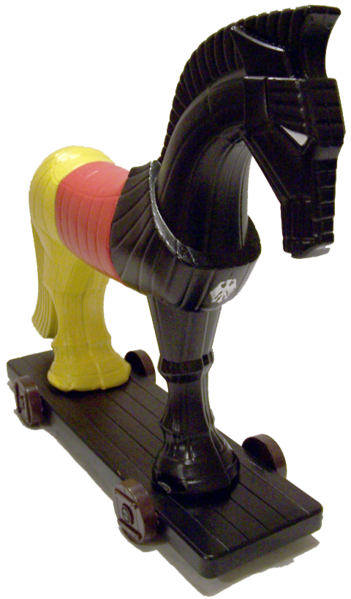
\includegraphics[height=0.7\textheight]{img/trojaner.png}
  \end{figure}
\end{frame}

\begin{frame}
    \frametitle{Chaos Computer Club}
    \begin{itemize}
      \item<1-> Chaos Computer Club Dresden (\url{http://c3d2.de})
          \note{}
      \item<2-> Datenspuren: 13./14.09.2014 \url{http://datenspuren.de}
      \item<3-> Podcasts (\url{http://pentamedia.de})
      \item<4-> Chaos macht Schule
    \end{itemize}
\end{frame}

\section{Datenschutz}
\subsection{}

\begin{frame}
    \frametitle{Bundespräsident Gauck zur NSA-Überwachung}
    \begin{center}
      "`Wir wissen z.B., dass es nicht so ist, wie bei der Stasi und dem KGB, dass es dicke Aktenbände gibt, wo unsere Gesprächsinhalte alle aufgeschrieben und schön abgeheftet sind. Das ist es nicht."'
      \end{center}
\end{frame}

\begin{frame}
    \frametitle{Stasi vs. NSA}
    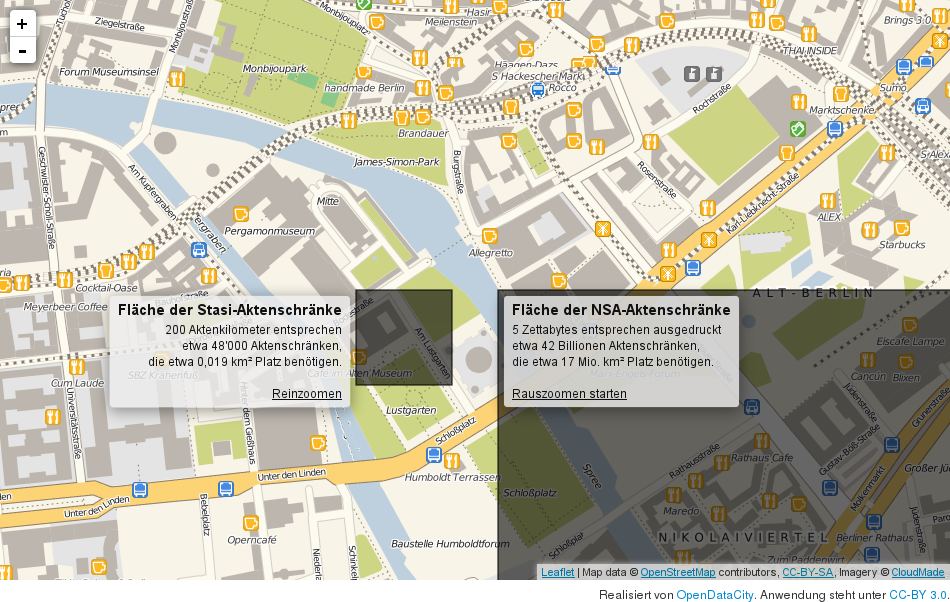
\includegraphics[height=0.7\textheight]{img/akten1.png}
\end{frame}

\begin{frame}
    \frametitle{Stasi vs. NSA}
    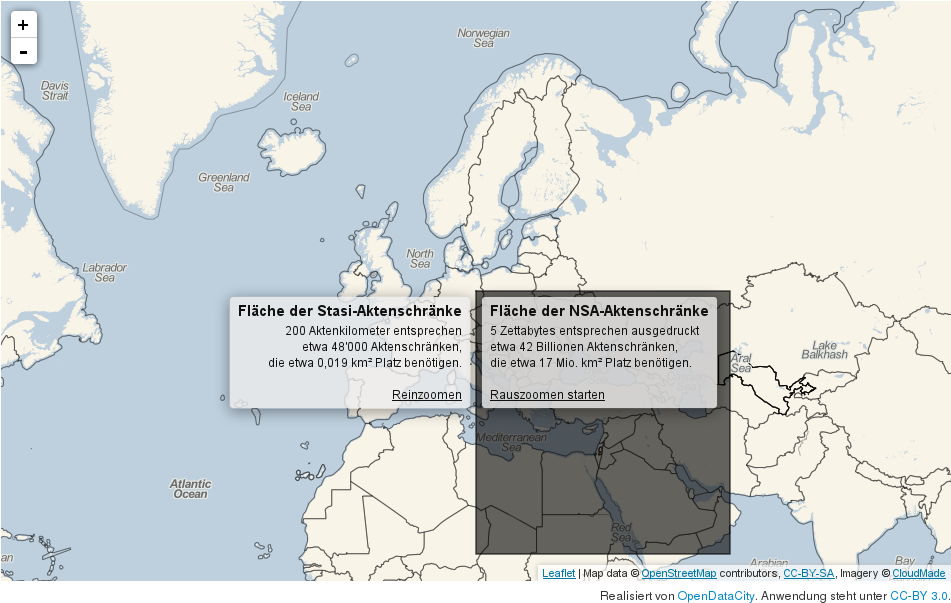
\includegraphics[height=0.7\textheight]{img/akten2.png}
\end{frame}

\begin{frame}
    \frametitle{Merkels Handy}
    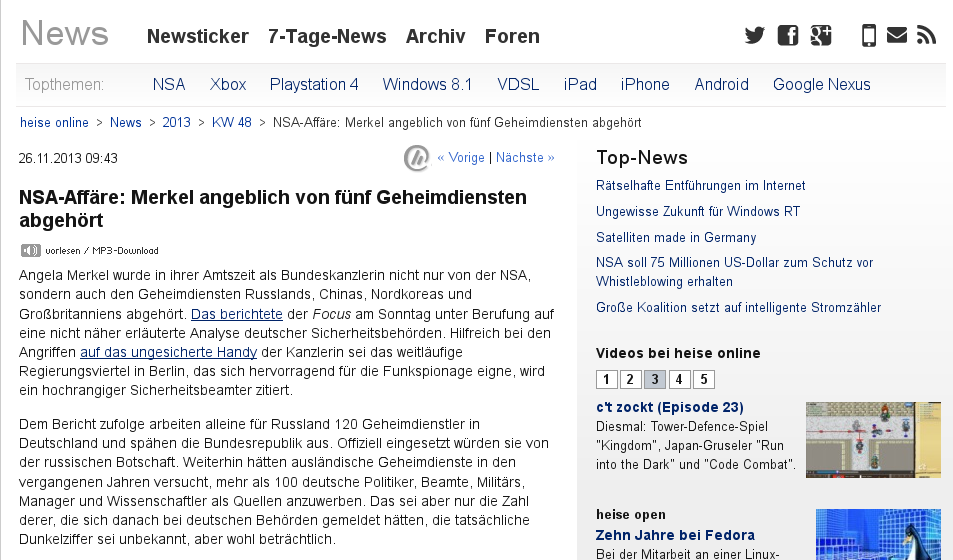
\includegraphics[height=0.7\textheight]{img/heise-merkel.png}
\end{frame}

\begin{frame}
    \frametitle{Wem nützen meine Daten?}
    \begin{itemize}
      \item<2-> Unternehmen
        \begin{itemize}
          \item<3-> (Zielgerichtete) Werbung
          \item<4-> Tracking
        \end{itemize}
      \item<5-> Staat, Geheimdienste
        \begin{itemize}
          \item<6-> Terrorismusbekämpfung? Kinderpornographie?
          \item<7-> => Kontrolle, Wirtschaftsspionage
        \end{itemize}
      \item<8->Meine Mitmenschen
    \end{itemize}
\end{frame}

\begin{frame}
    \frametitle{Wie schütze ich mich?}
    \begin{itemize}
      \item<1-> technisch
      \item<2-> Verhalten
    \end{itemize}
\end{frame}

\section{Kommunikation}
\subsection{}

\begin{frame}
    \frametitle{Wie kommunizieren wir im Internet?}
    \begin{center}
      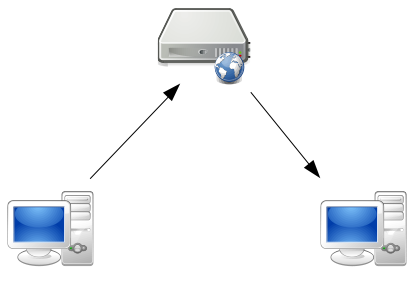
\includegraphics[height=5cm]{img/c-s.png}
    \end{center}
\end{frame}

\begin{frame}
    \frametitle{Föderation}
    \begin{center}
      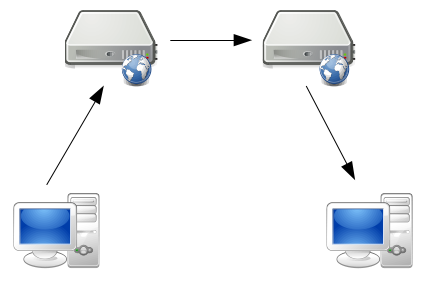
\includegraphics[height=5cm]{img/fed.png}
    \end{center}
\end{frame}

\begin{frame}
    \frametitle{P2P}
    \begin{center}
      
\includegraphics[width=7cm]{img/direkt.png}
    \end{center}
\end{frame}

\begin{frame}
    \frametitle{P2P: Praxis-Beispiel: https://palava.tv}
    \begin{center}
      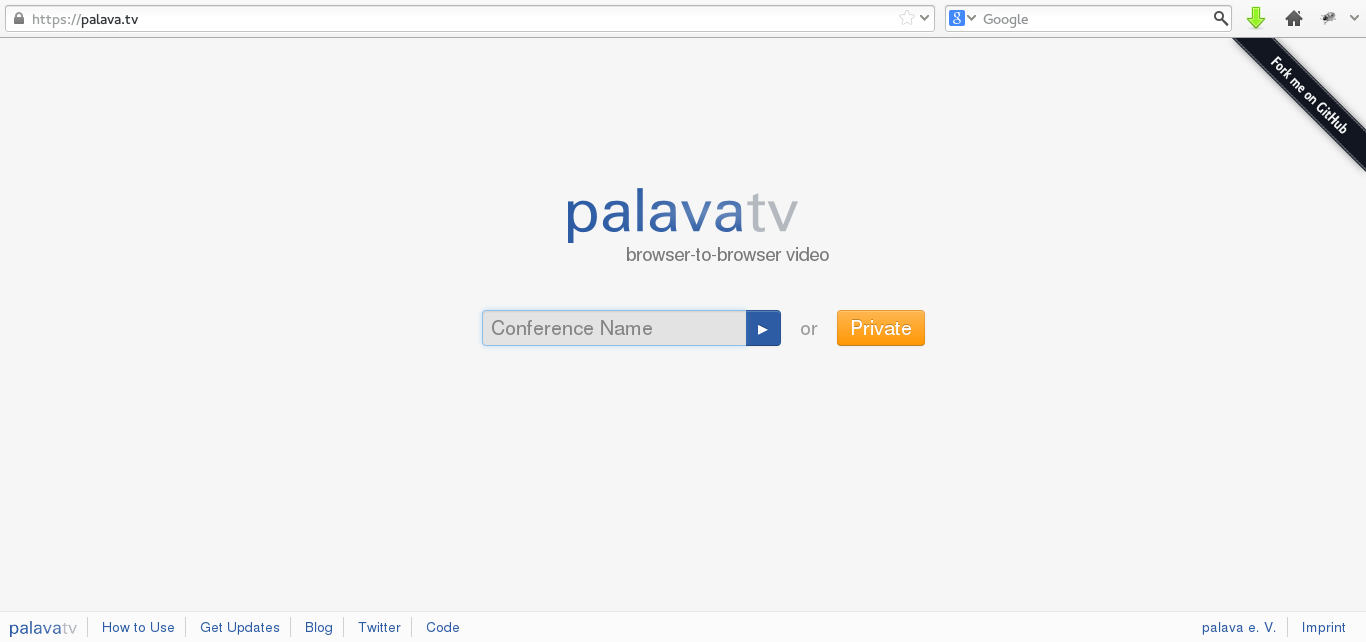
\includegraphics[width=\linewidth]{img/palava.png}
    \end{center}
\end{frame}

\begin{frame}
    \frametitle{Was ist zu schützen?}
    \begin{center}
      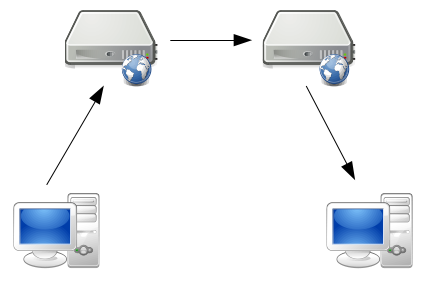
\includegraphics[height=5cm]{img/fed.png}
    \end{center}
\end{frame}

\begin{frame}
    \frametitle{Was ist zu schützen?}
    \begin{center}
      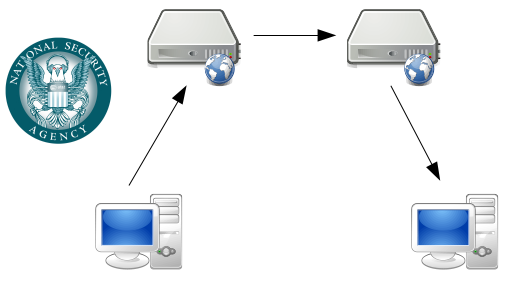
\includegraphics[height=5cm]{img/fed-bad-guy.png}
    \end{center}
\end{frame}

\begin{frame}
    \frametitle{Tempora}
    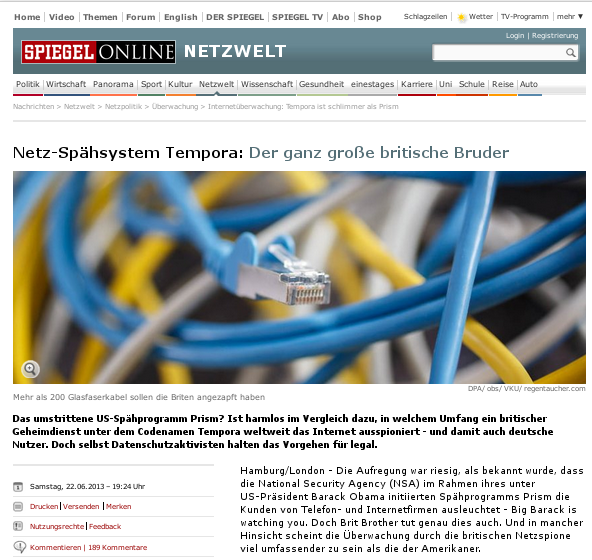
\includegraphics[height=0.7\textheight]{img/spiegel-tempora.png}
\end{frame}

\begin{frame}
    \frametitle{Prism}
    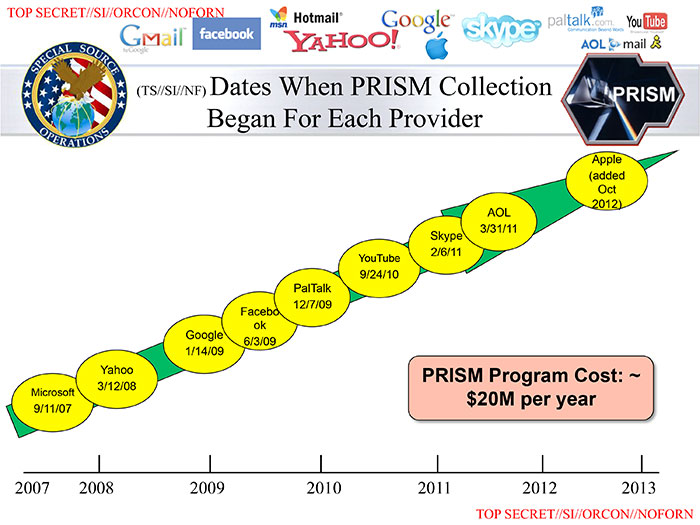
\includegraphics[height=0.7\textheight]{img/prism.jpg}
\end{frame}

\begin{frame}
    \frametitle{Was ist zu schützen?}
    \begin{center}
      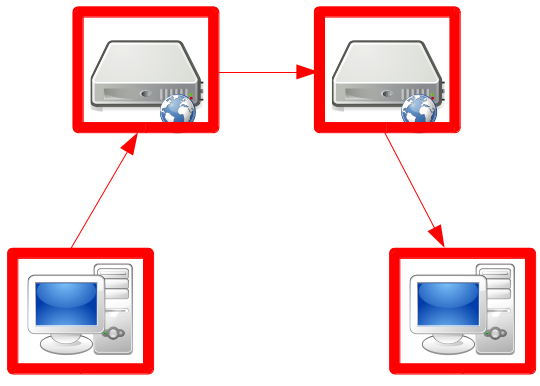
\includegraphics[height=5cm]{img/fed-none.png}
    \end{center}
\end{frame}

\section{Geräte}
\subsection{}

\begin{frame}
    \frametitle{Wie schütze ich meinen Computer?}
    \begin{itemize}
      \item (Virenscanner)
      \item Firewall
      \item Aktuelle und vertrauenswürdige Software
    \end{itemize}
\end{frame}

\begin{frame}
    \frametitle{Wie schütze ich mein Smartphone?}
    \begin{itemize}
      \item Permissions
      \item Firewall (z.B. AFwall+: https://f-droid.org/repository/browse/?fdid=dev.ukanth.ufirewall)
      \item Aktuelle und vertrauenswürdige Software
      \item Alternativer Appstore: f-droid.org
    \end{itemize}
\end{frame}

\begin{frame}
    \frametitle{Vertrauenswürdige Software?}
    \begin{center}\Large
        Einer Software, die nicht quelloffen ist, kann man nicht vertrauen
    \end{center}
\end{frame}

\begin{frame}
    \frametitle{Open Source Software}
    \begin{center}
      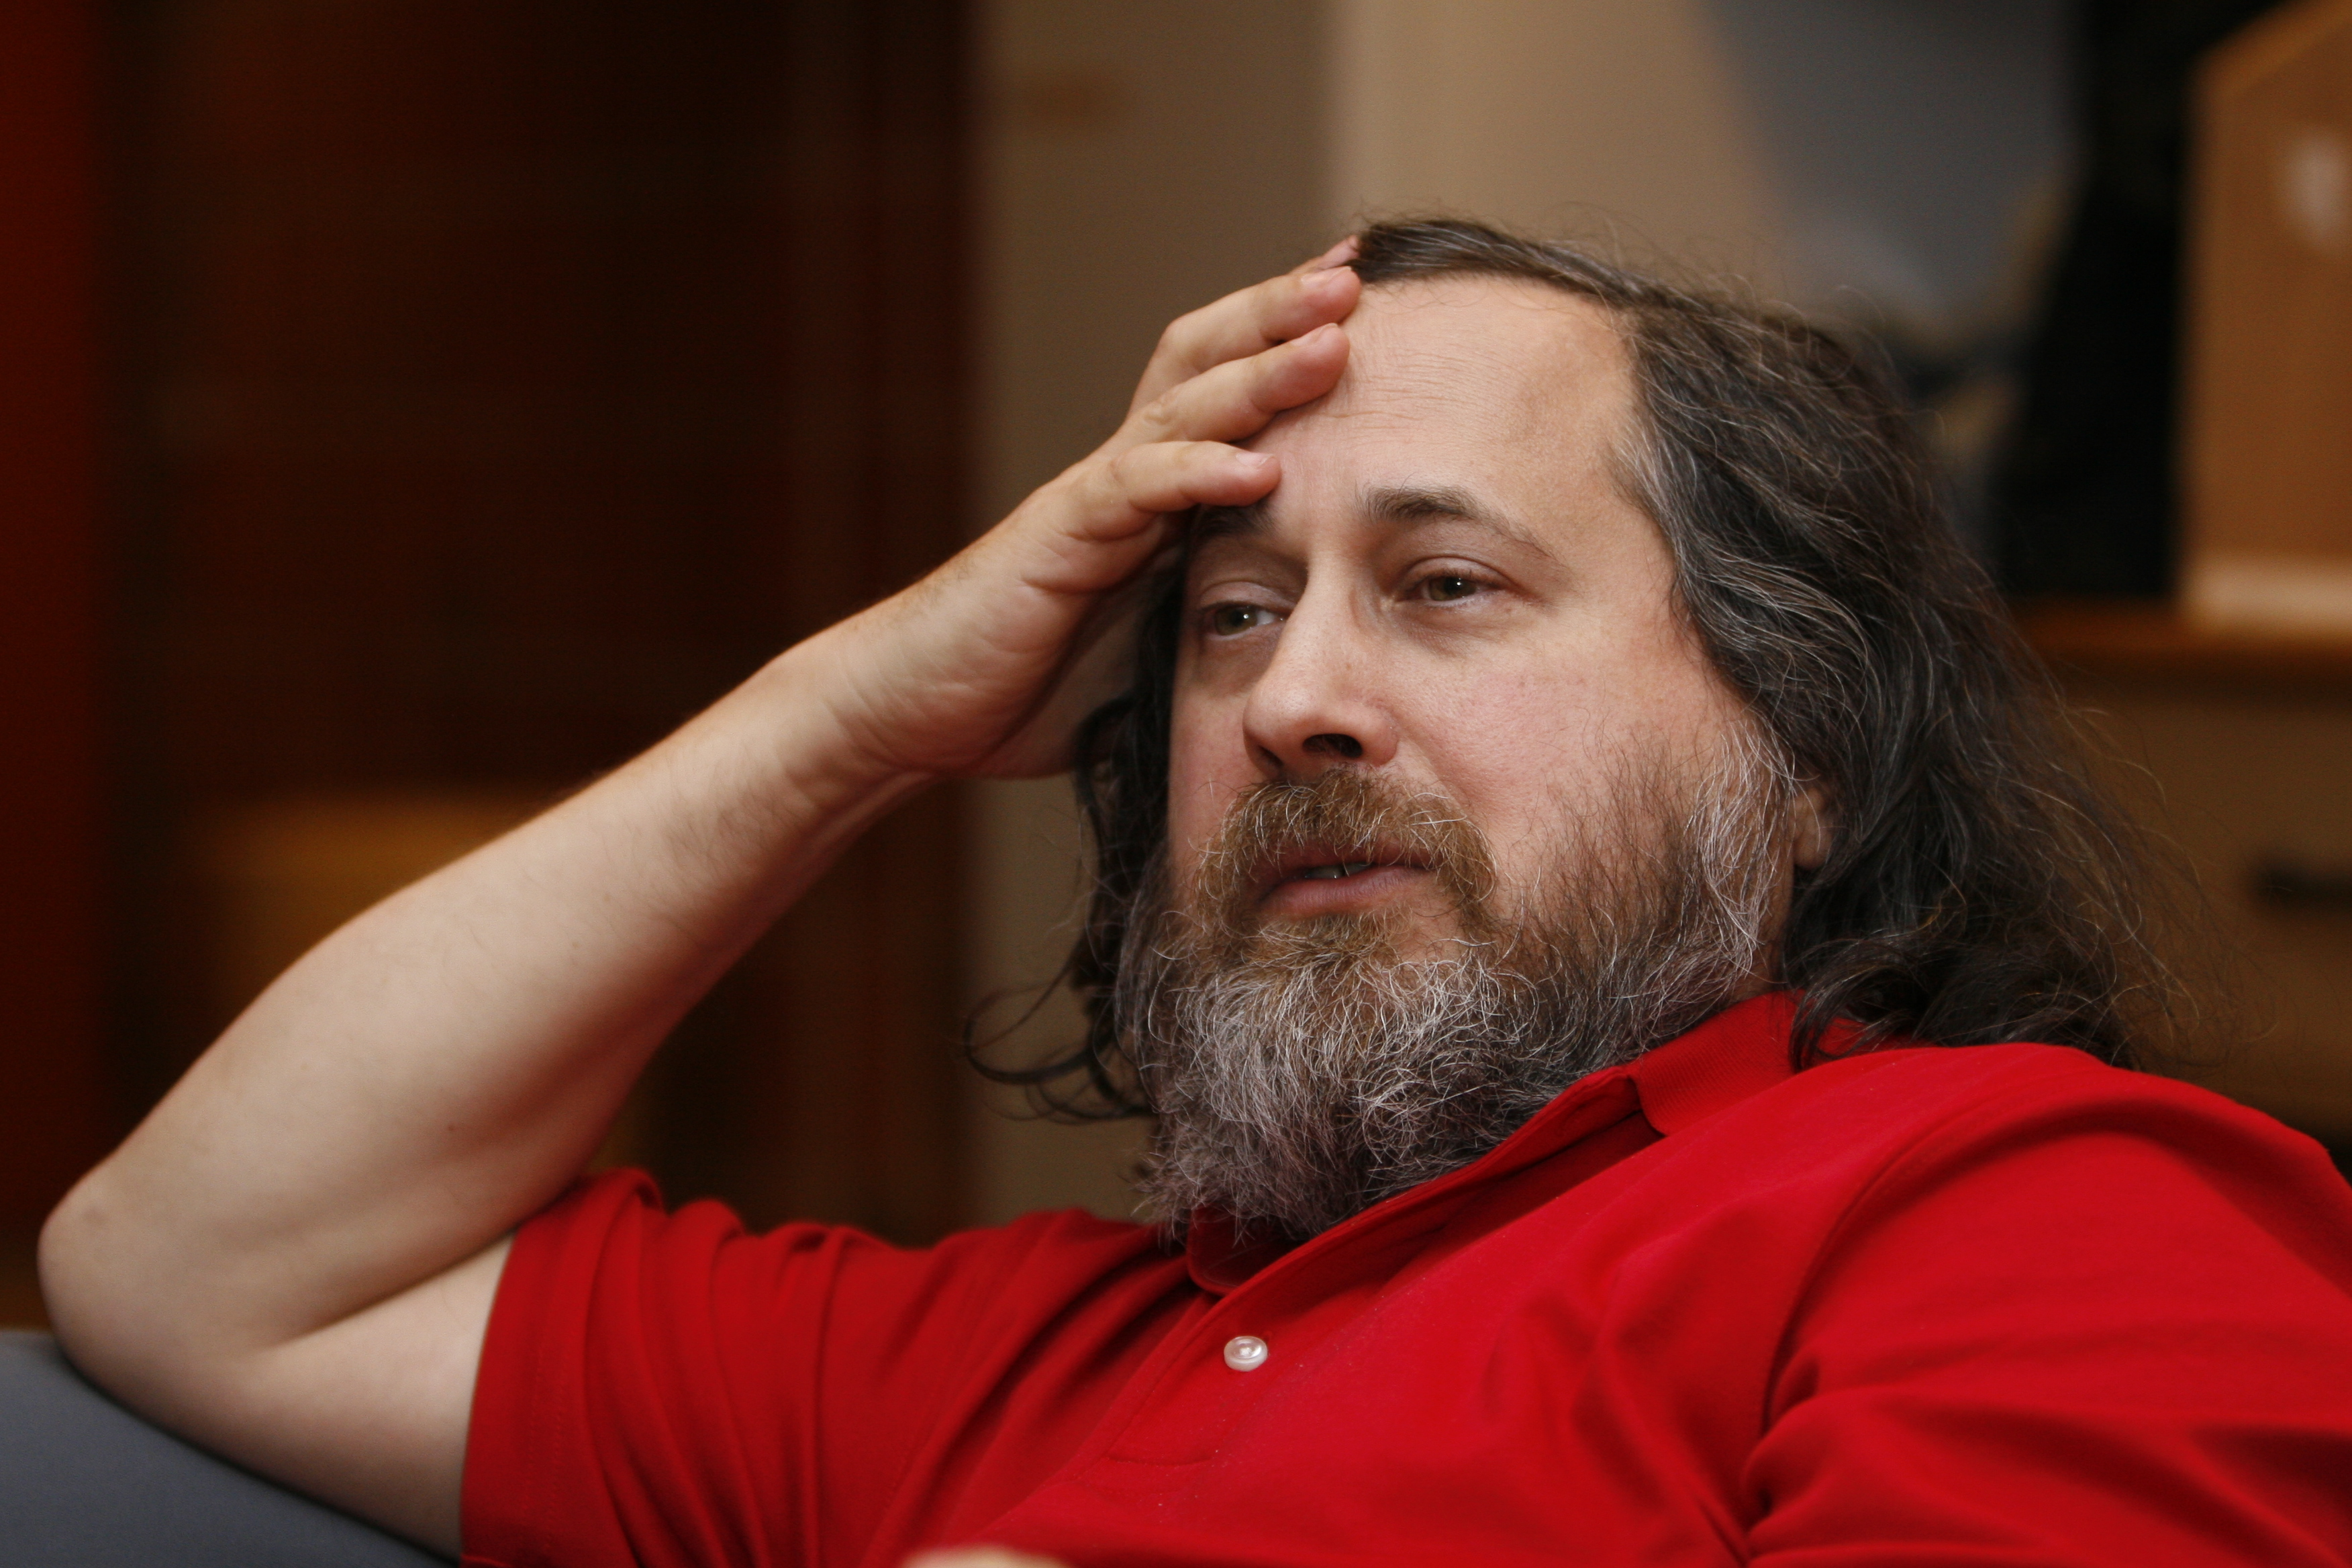
\includegraphics[height=0.7\textheight]{img/stallman.jpg}
      \\{\small \href{http://tekniskbeta.no/frie-cc-bilder-av-richard-stallman/}{Foto}: \href{http://creativecommons.org/licenses/by/3.0/no/}{\cc{by}} Anders Brenna}
    \end{center}
\end{frame}

\begin{frame}
    \frametitle{Freie Software}
    \begin{itemize}
      \item Firefox
      \item Thunderbird
      \item LibreOffice
      \item Pidgin
      \item Evince/Okular
      \item Gimp
      \item VLC
    \end{itemize}
\end{frame}

\begin{frame}
    \frametitle{Freie Software}
    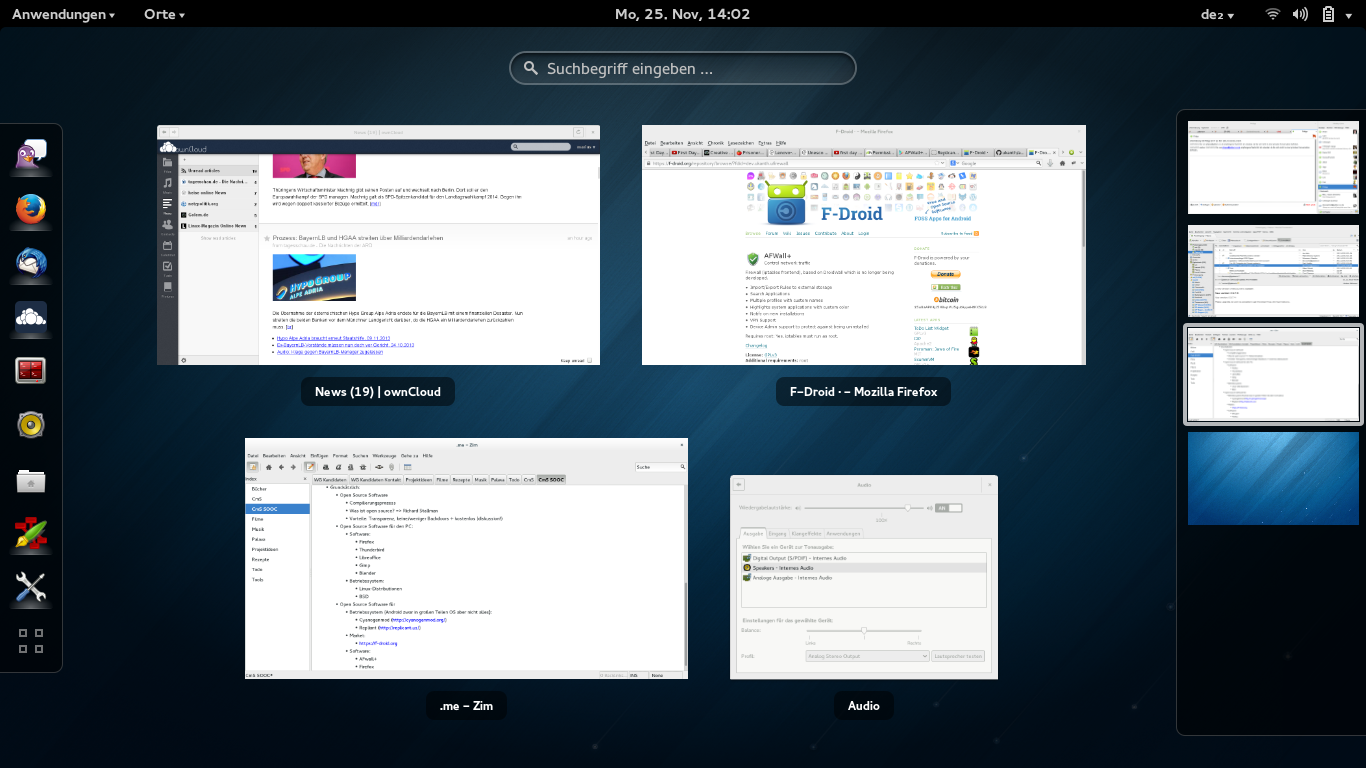
\includegraphics[height=0.7\textheight]{img/gnome.png}
\end{frame}

\begin{frame}
    \frametitle{Freie Software}
    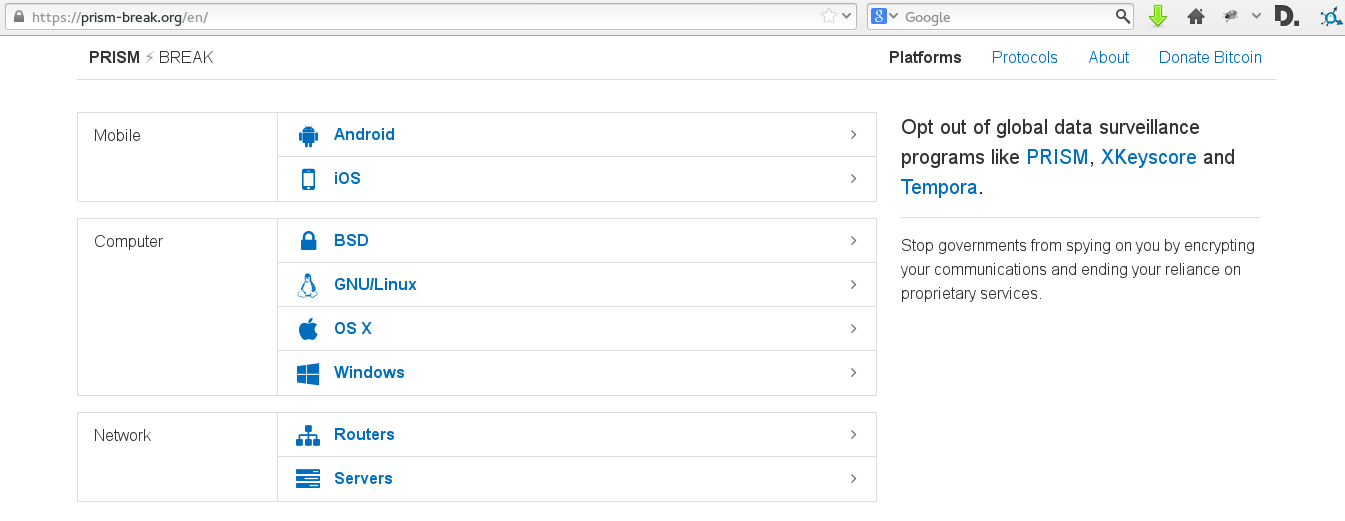
\includegraphics[height=0.7\textheight]{img/prism-break1.png}
\end{frame}

\begin{frame}
    \frametitle{Freie Software}
    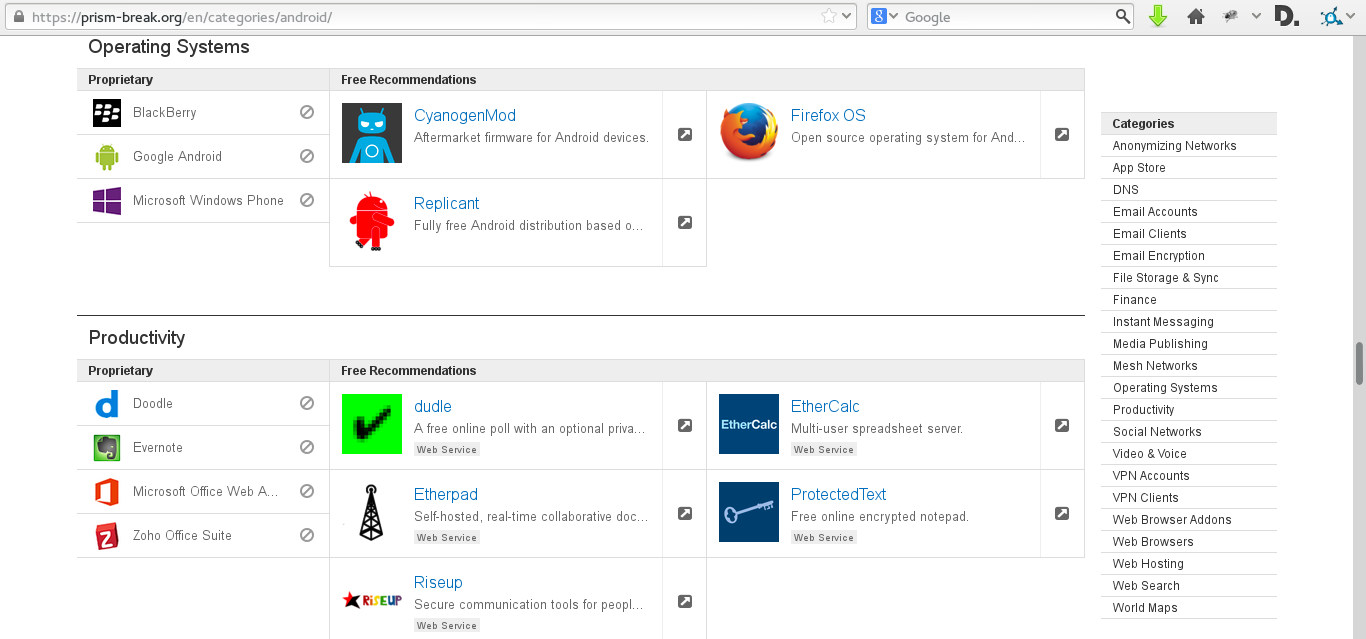
\includegraphics[height=0.7\textheight]{img/prism-break2.png}
\end{frame}

\begin{frame}
    \frametitle{Zusammenfassung}
    \begin{itemize}
      \item Computer/Handy absichern
      \item Open Source Software verwenden
    \end{itemize}
\end{frame}

\section{Verschlüsselung I}
\subsection{}

\begin{frame}
    \frametitle{Was ist zu schützen?}
    \begin{center}
      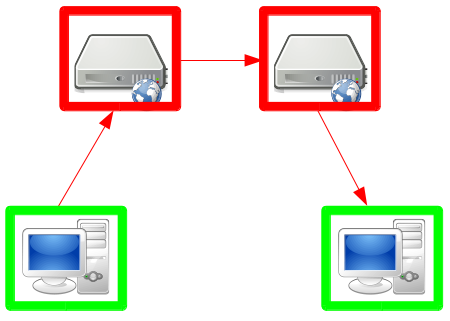
\includegraphics[height=5cm]{img/fed-clients.png}
    \end{center}
\end{frame}

\begin{frame}
    \frametitle{Verschlüsselung: Analogie}
    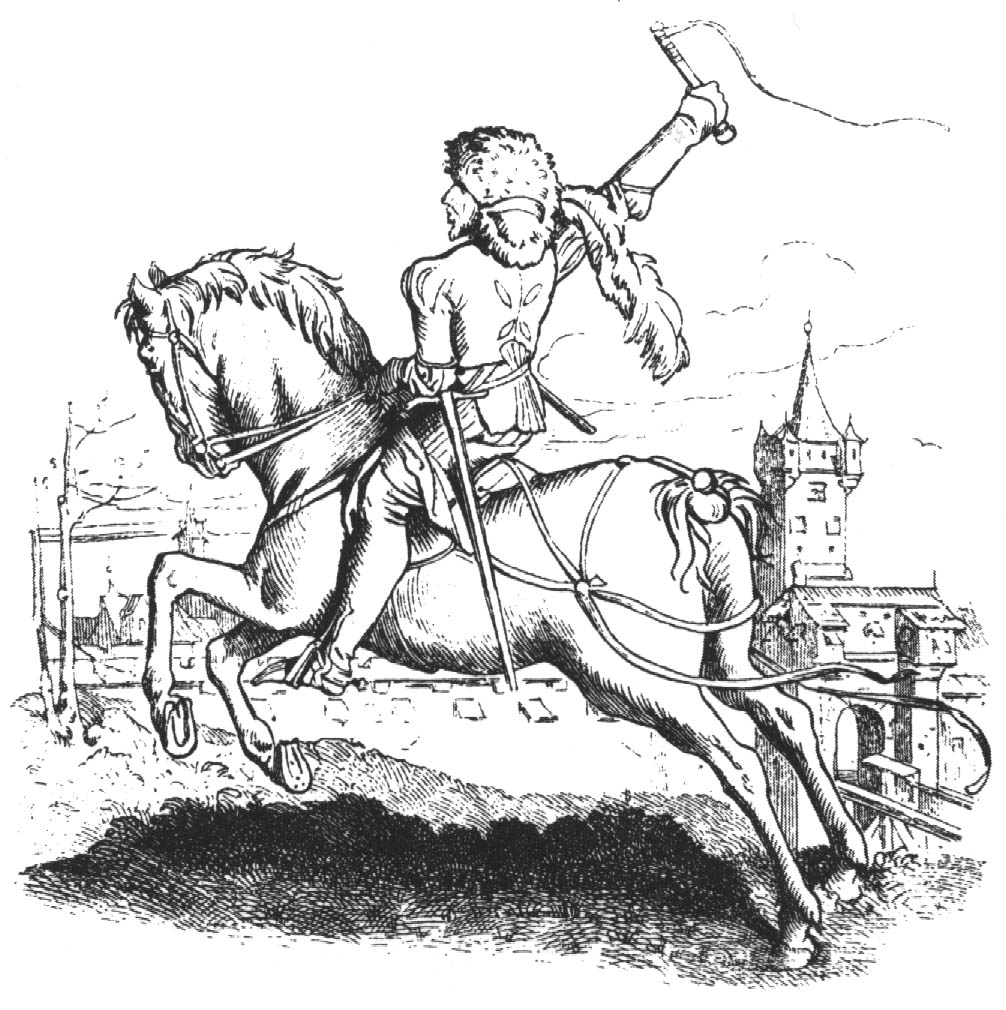
\includegraphics[height=0.7\textheight]{img/bote.jpg}
    {\\ \small \href{http://commons.wikimedia.org/wiki/File:Reitbote.jpg}{Grafik}: \href{http://creativecommons.org/licenses/by-sa/2.5/deed.en}{\cc{by-sa}} Ronald Preuss}
\end{frame}

\begin{frame}
    \frametitle{Verschlüsselung: Asymmetrische}
    \includegraphics[height=0.7\textheight]<2->{img/asym_encryption.png}
\end{frame}

\begin{frame}
    \frametitle{SSL / TLS}
    \begin{itemize}
      \item<2-> SSL = Secure Socket Layer
      \item<3-> eingesetzt im Web, Mail, ...
    \end{itemize}
\end{frame}

\begin{frame}
    \frametitle{SSL im Browser}
    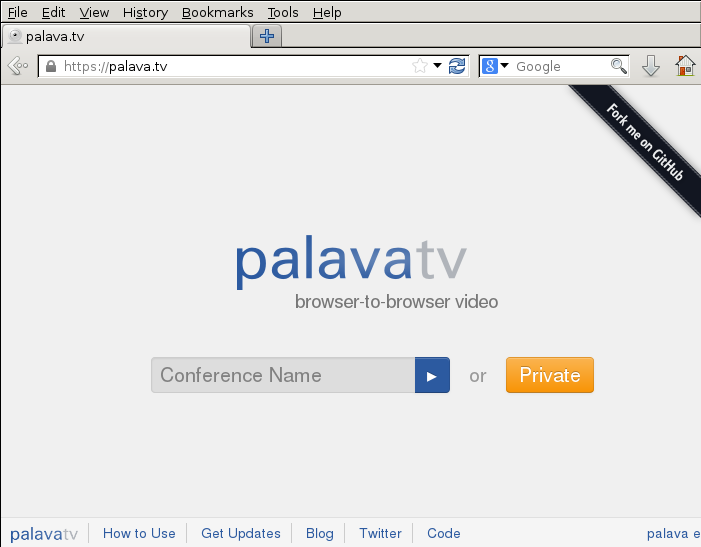
\includegraphics[height=0.7\textheight]{img/ssl_verified.png}
\end{frame}

\begin{frame}
    \frametitle{SSL im Browser}
    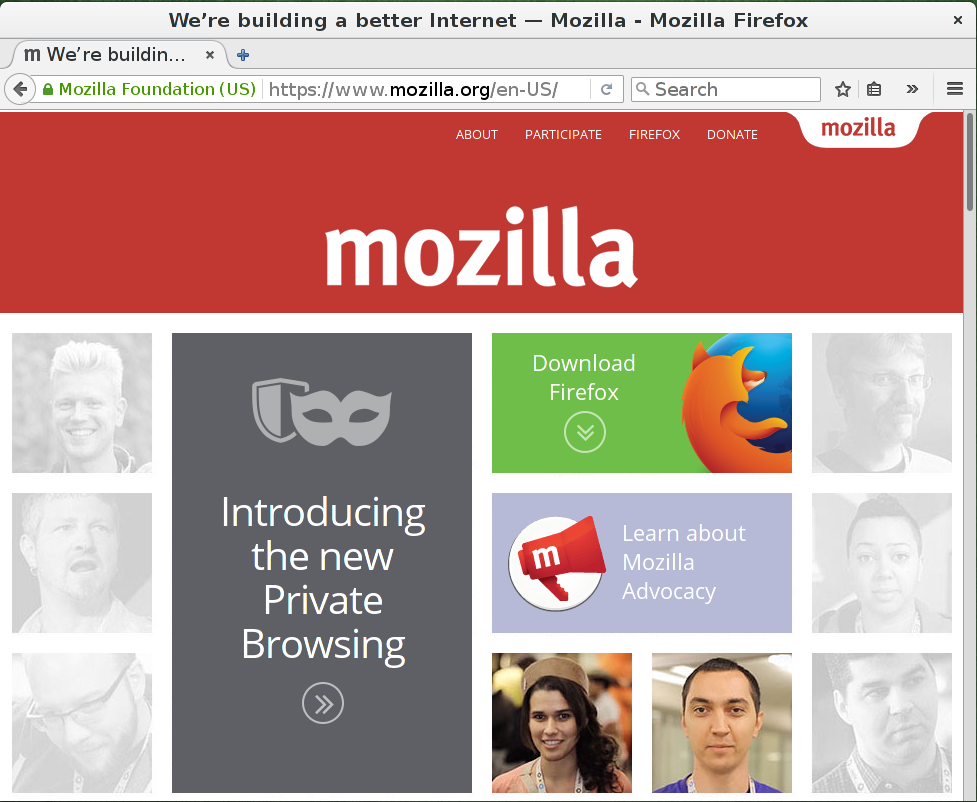
\includegraphics[height=0.7\textheight]{img/ssl_special.png}
\end{frame}

\begin{frame}
    \frametitle{SSL im Browser}
    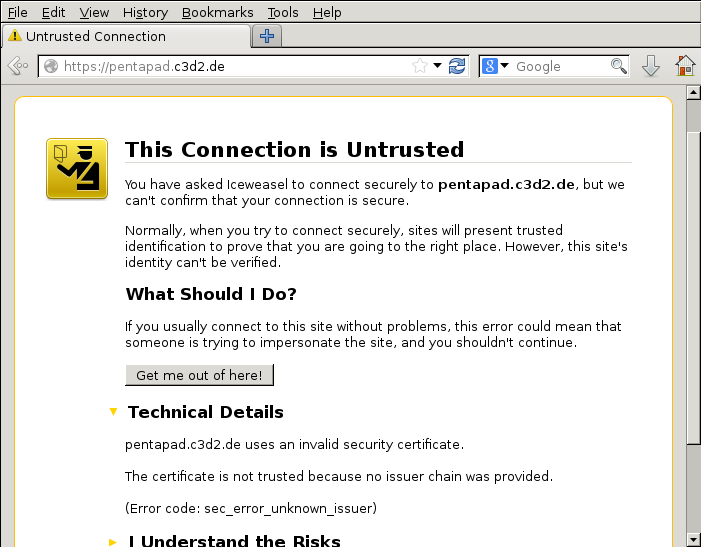
\includegraphics[height=0.7\textheight]{img/ssl_unverified.png}
\end{frame}

\begin{frame}
    \frametitle{Zertifizierungsstellen}
    \begin{center}
      \includegraphics[height=5cm]<2->{img/zertifikate.png}
    \end{center}
\end{frame}

\begin{frame}
  \frametitle{HTTPS Everywhere}
    \begin{center}
      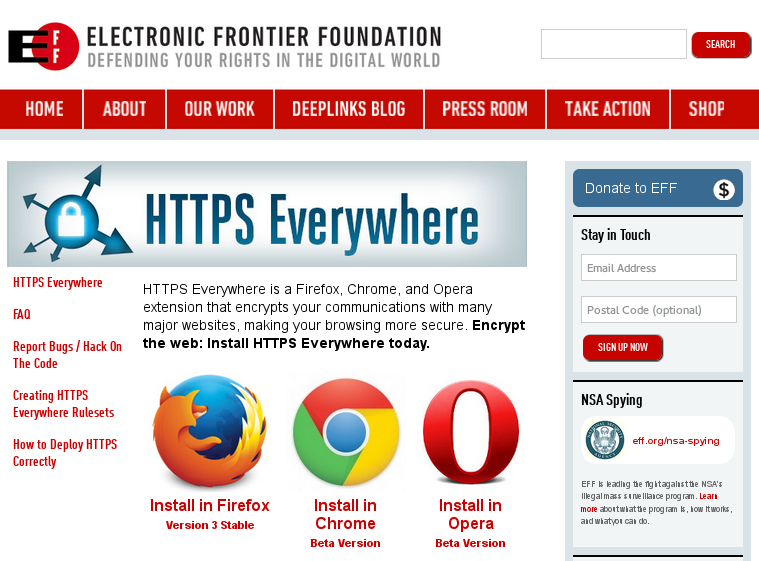
\includegraphics[height=5cm]{img/https-everywhere.png}
    \end{center}
\end{frame}

\section{Anonymität}
\subsection{}

\begin{frame}
  \frametitle{Vorratsdatenspeicherung (USA)}
    \begin{center}
      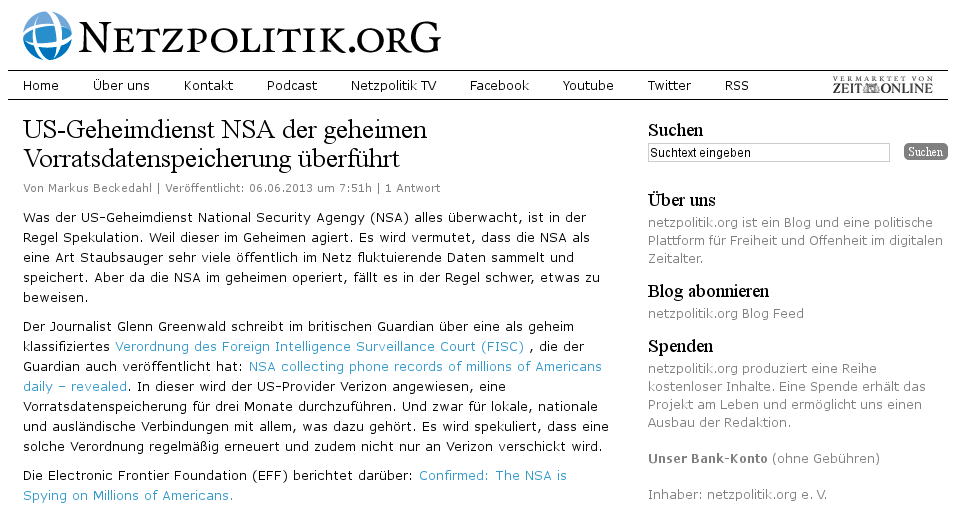
\includegraphics[height=5cm]{img/netzpolitik-verizon.png}
    \end{center}
\end{frame}

\begin{frame}
  \frametitle{Vorratsdatenspeicherung (Deutschland)}
    \begin{center}
      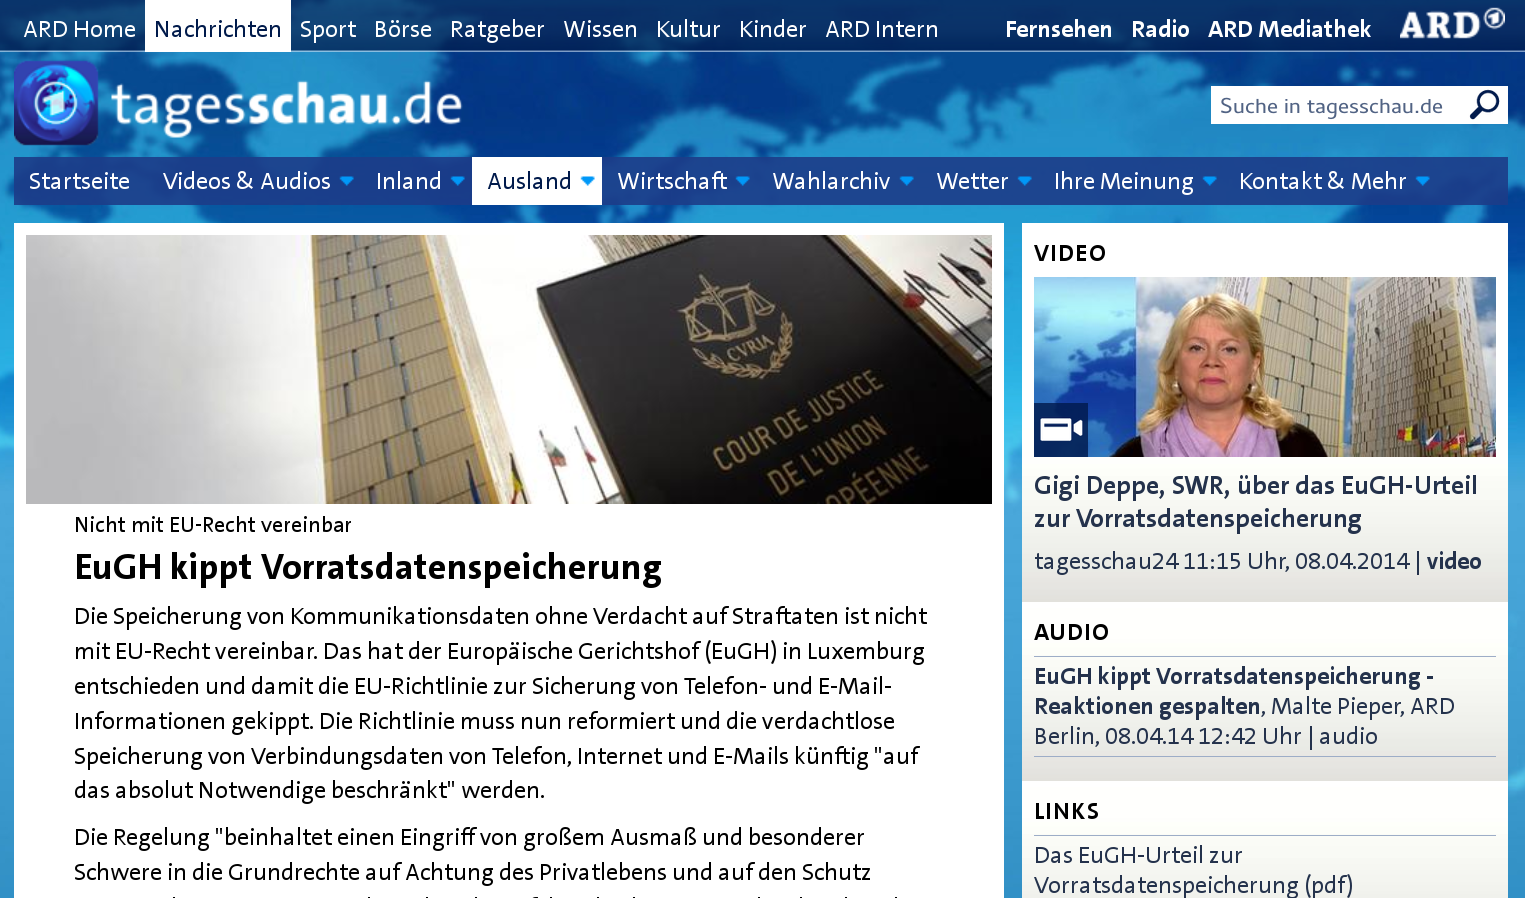
\includegraphics[height=5cm]{img/tagesschau-vds.png}
    \end{center}
\end{frame}

\begin{frame}
  \frametitle{Metadaten}
    \begin{center}
      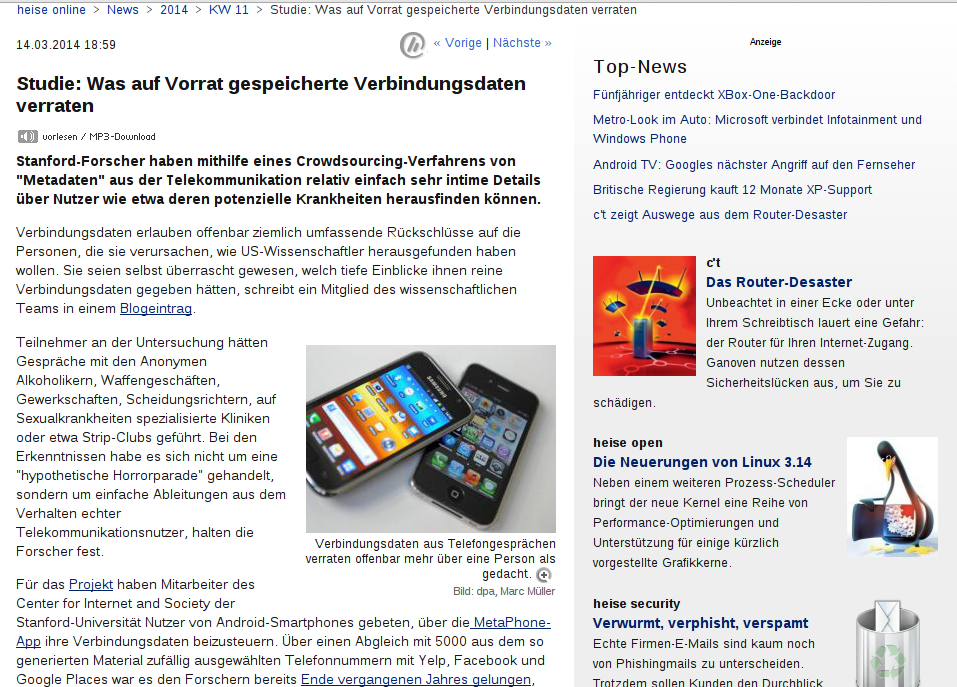
\includegraphics[height=5cm]{img/metadaten_studie.png}
    \end{center}
\end{frame}

\begin{frame}
    \frametitle{Metadaten}
    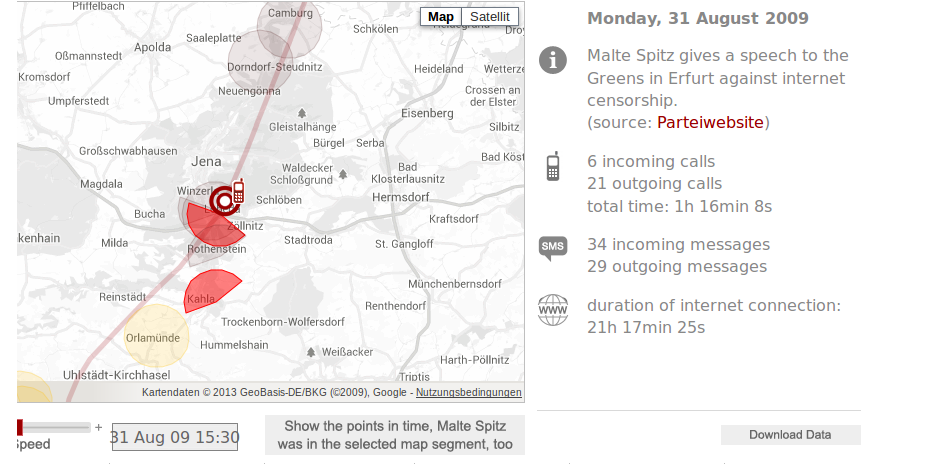
\includegraphics[height=0.7\textheight]{img/maltespitz.png}
\end{frame}

\begin{frame}
    \frametitle{Tor}
    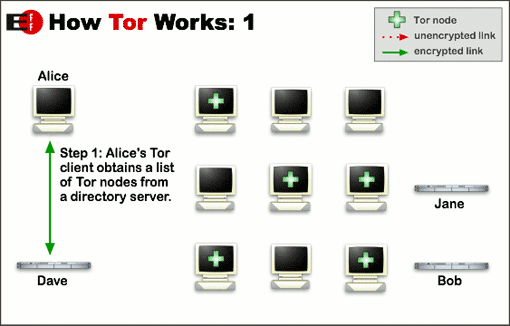
\includegraphics[height=0.7\textheight]{img/tor1.png}
    \\{\small \href{https://www.torproject.org/images/htw1.png}{Grafik}: \href{https://creativecommons.org/licenses/by/3.0/us/}{\cc{by}} The Tor Project}
\end{frame}

\begin{frame}
    \frametitle{Tor}
    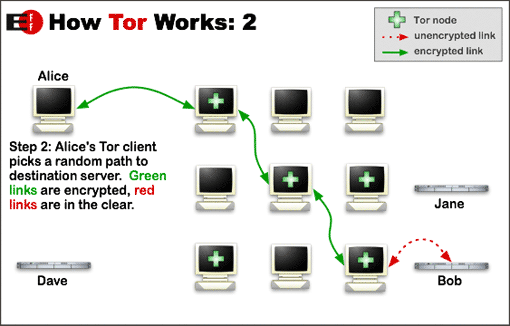
\includegraphics[height=0.7\textheight]{img/tor2.png}
    \\{\small \href{https://www.torproject.org/images/htw2.png}{Grafik}: \href{https://creativecommons.org/licenses/by/3.0/us/}{\cc{by}} The Tor Project}
\end{frame}

\begin{frame}
    \frametitle{Tor}
    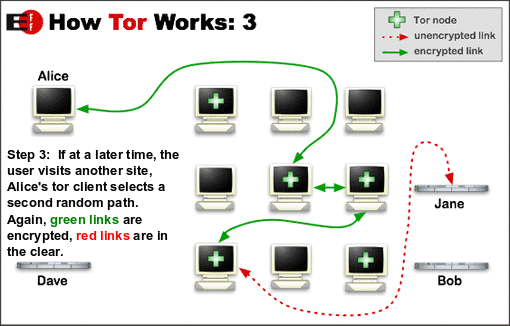
\includegraphics[height=0.7\textheight]{img/tor3.png}
    \\{\small \href{https://www.torproject.org/images/htw3.png}{Grafik}: \href{https://creativecommons.org/licenses/by/3.0/us/}{\cc{by}} The Tor Project}
\end{frame}

\begin{frame}
  \frametitle{Tor}
  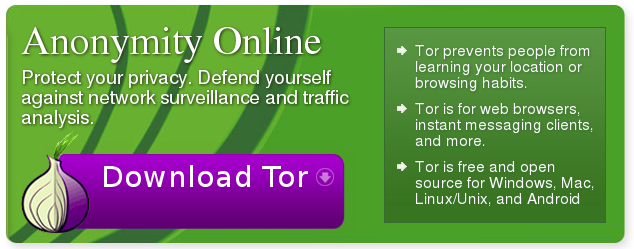
\includegraphics[height=0.5\textheight]{img/tor-banner.png}
\end{frame}

\begin{frame}
    \frametitle{Zensur}
    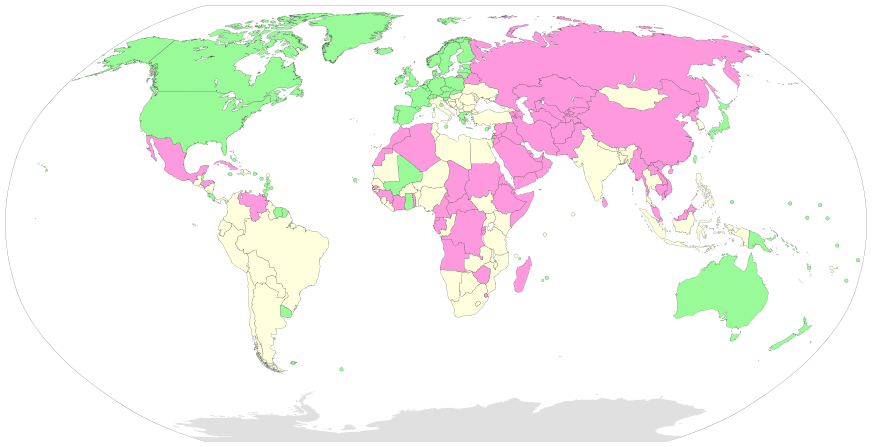
\includegraphics[height=0.7\textheight]{img/zensur.png}
    \\{\small \href{http://upload.wikimedia.org/wikipedia/commons/5/51/RWB-PressFreedomIndex2013-WorldMap.svg}{Grafik}: \href{http://creativecommons.org/licenses/by-sa/3.0/deed.en}{\cc{by-sa}} Jeff Ogden (W163)}
\end{frame}

\begin{frame}
    \frametitle{Tor in der Türkei}
    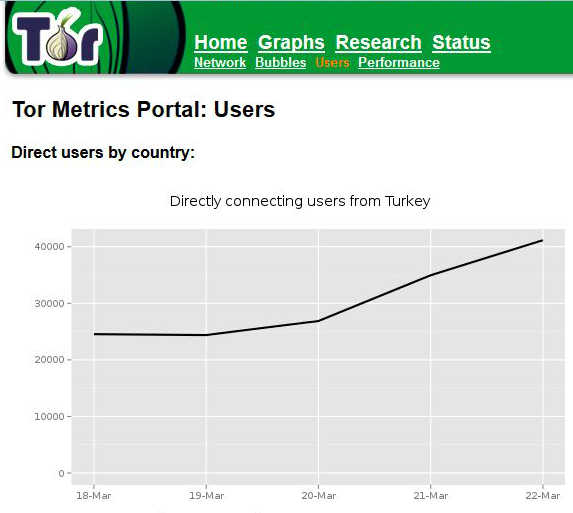
\includegraphics[height=0.7\textheight]{img/tor-tuerkei.jpg}
\end{frame}

\begin{frame}
    \frametitle{Anonymität unter Vollüberwachung}
    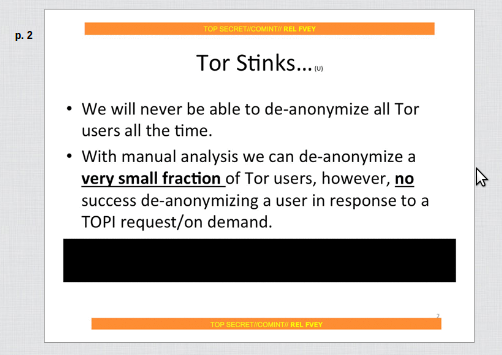
\includegraphics[height=0.7\textheight]{img/torstinks.png}
\end{frame}

\begin{frame}
    \frametitle{Zusammenfassung}
    \begin{itemize}
      \item SSL nutzen (mit HTTPS Everywhere)
      \item Anonymität wahren (mit Tor)
    \end{itemize}
\end{frame}


\begin{frame}
    \frametitle{Was ist zu schützen?}
    \begin{center}
      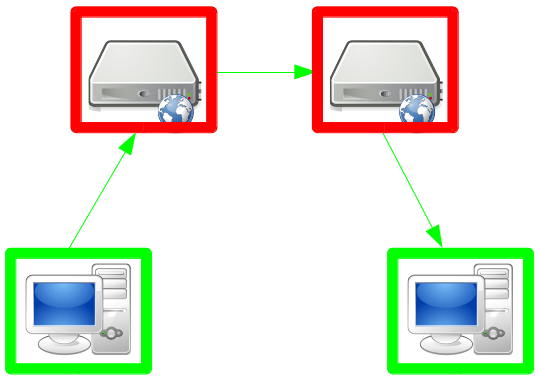
\includegraphics[height=5cm]{img/fed-clients-comm.png}
    \end{center}
\end{frame}

\begin{frame}
    \frametitle{Was ist zu schützen?}
    \begin{center}
      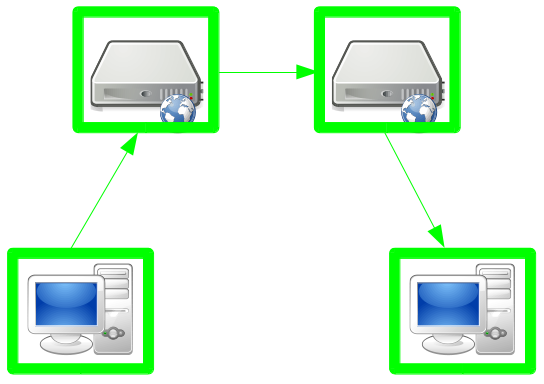
\includegraphics[height=5cm]{img/fed-all.png}
    \end{center}
\end{frame}

\section{Unternehmen}
\subsection{}

\begin{frame}
    \frametitle{Was ist zu schützen?}
    \begin{center}
      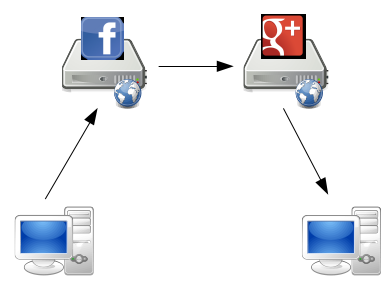
\includegraphics[height=5cm]{img/fed-social.png}
    \end{center}
\end{frame}

\begin{frame}
    \frametitle{Metadaten - Lightbeam}
    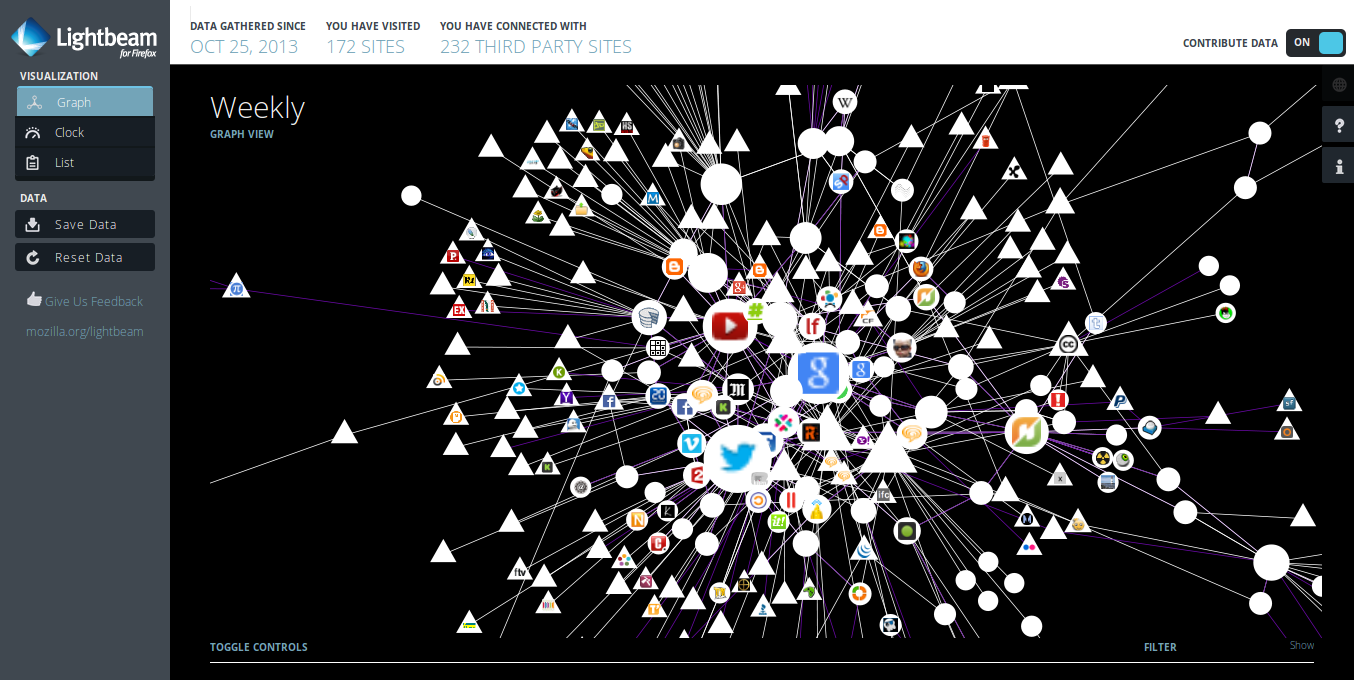
\includegraphics[height=0.7\textheight]{img/lightbeam.png}
  \\{\small \href{http://www.flickr.com/photos/8517757@N03/10538205035/in/photolist-h4e4dg}{Grafik:} \href{http://creativecommons.org/licenses/by-sa/3.0/deed.en}{\cc{by-sa}} Clint Lalonde}
\end{frame}

\begin{frame}
    \frametitle{Ich will etwas vom Server I}
    \begin{center} 
        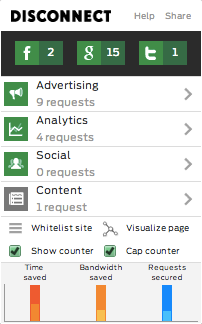
\includegraphics[height=0.5\textheight]{img/disconnect.png} \\
        \Large Disconnect.me 
    \end{center}
\end{frame}

\begin{frame}
    \frametitle{Ich will etwas vom Server II}
    \begin{itemize}
      \item<2-> Datensparsamkeit
      \item<3-> Werden echte Daten gebraucht?
          \begin{itemize}
            \item<4-> Pseudonymität
            \item<5-> mailinator.com (Wegwerf-Email-Adresse)
            \item<6-> frank-geht-ran.de (Wegwerf-Telefonnummer)
            \item<7-> bugmenot.com (Fake Accounts)
          \end{itemize}
    \end{itemize}
\end{frame}

\begin{frame}
  \frametitle{Ich will etwas von einem anderen Nutzer}
    \begin{center}
      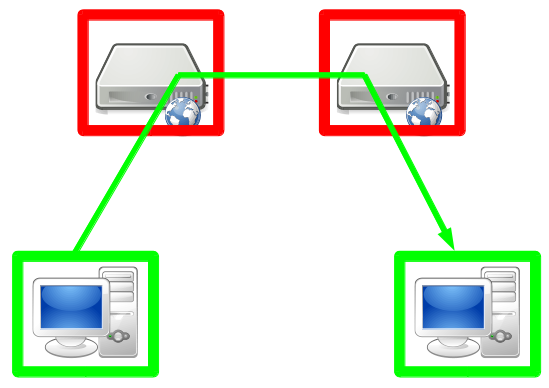
\includegraphics[height=5cm]{img/fed-end-to-end.png}
    \end{center}
\end{frame}

\begin{frame}
    \frametitle{Ende-zu-Ende-Verschlüsselung I}
    \begin{itemize}\Large
      \item Email: GPG = Gnu Privacy Guard
      \item Thunderbird: Enigmail
      \item Outlook: Gpg4win
      \item Apple Mail: GPGTools
      \item Web: Mailvelope (Firefox, Chrome)
    \end{itemize}
\end{frame}

\begin{frame}
  \frametitle{Ende-zu-Ende-Verschlüsselung II}
  \begin{itemize}
    \item<2-> OTR für Jabber:
      \begin{itemize}
        \item Pidgin mit OTR-Plugin für Linux und Windows
        \item GibberBot oder Xabber für Android
        \item Adium für Mac, ChatSecure für iOS
      \end{itemize}
    \item<3-> palava.tv für Videotelefonie
    \item<4-> Redphone für Handytelefonate (Android)
    \item<5-> TextSecure für Nachrichten (Android)
  \end{itemize}
\end{frame}

\begin{frame}
  \frametitle{Authentifizierung}
    \begin{center}
      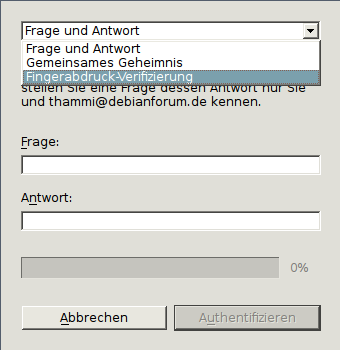
\includegraphics[height=5cm]{img/auth.png}
    \end{center}
\end{frame}

\begin{frame}
  \frametitle{TextSecure}
    \begin{center}
      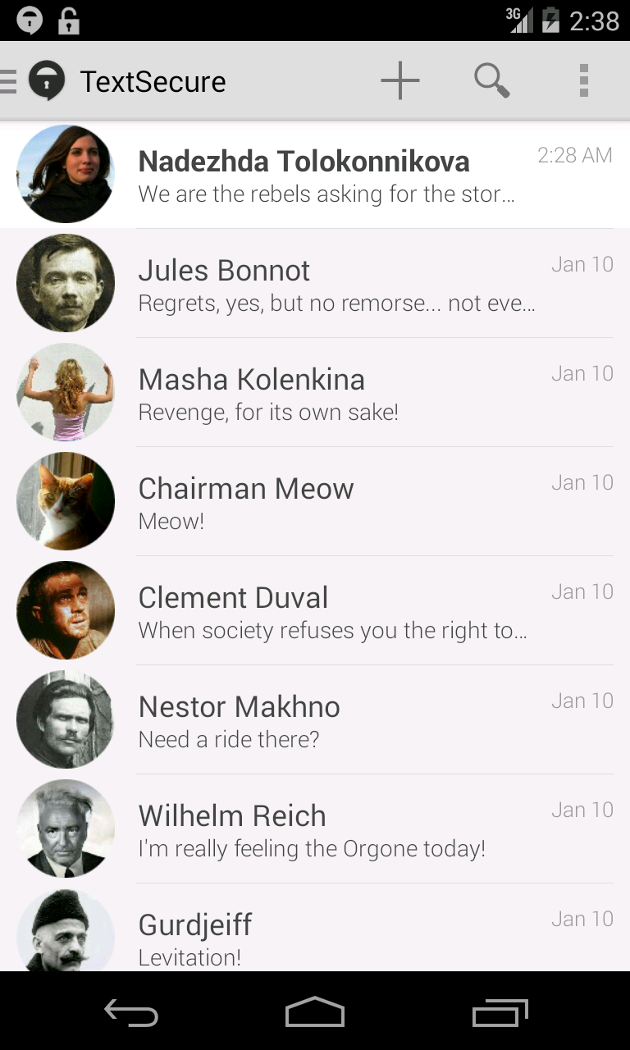
\includegraphics[height=6cm]{img/textsecure1.png}
      \hspace{0.5cm}
      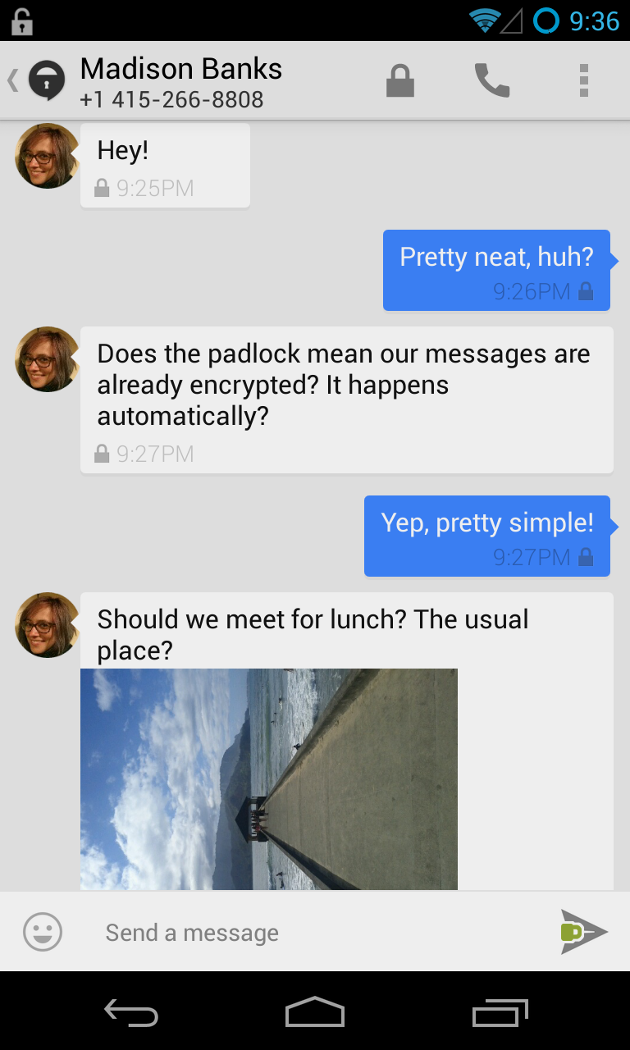
\includegraphics[height=6cm]{img/textsecure2.png}
    \end{center}
\end{frame}
 
\begin{frame}
    \frametitle{Zusammenfassung}
    \begin{itemize}
      \item Tracking-Daten loswerden mit Disconnect
      \item Datensparsamkeit / falsche Daten
      \item Ende-zu-Ende-Verschlüsselung
    \end{itemize}
\end{frame}

\begin{frame}
  \frametitle{Diskussion}
  \begin{center}
    {\Large Diskussion}\\
    \vspace{5mm} 
    \href{https://github.com/c3d2/cms-nsa}{Folien}: \href{https://creativecommons.org/licenses/by-sa/4.0/}{\cc{by-sa}} Marius Melzer \\
    \vspace{4mm}
    Twitter: @faraoso, Email und Jabber: marius@rasumi.net\\GPG-Fingerprint: 52DEFC3E\\
    \vspace{4mm}
    CMS Dresden: schule@c3d2.de
  \end{center}
\end{frame}

\end{document}
